\title{Midterm 3 for Algebra-Based Physics-1: Mechanics (PHYS135A-01)}
\author{Dr. Jordan Hanson - Whittier College Dept. of Physics and Astronomy}
\date{November 19th, 2017}
\documentclass[10pt]{article}
\usepackage[a4paper, total={18cm, 27cm}]{geometry}
\usepackage{outlines}
\usepackage[sfdefault]{FiraSans}
\usepackage{graphicx}

\begin{document}
\maketitle
\small
\section{Rotational Kinematics and Dynamics}
\begin{enumerate}
\item Express the following angles in radians: (a) $180^{\circ}$ (b) $90^{\circ}$ (c) $120^{\circ}$ (d) $270^{\circ}$ \\ \vspace{1cm}
\item A man spins a grindstone to sharpen a knife, and can accelerate the grindstone with a foot pedal.  Suppose the grindstone has a radius $r=5$ cm, and is spinning initially at 60 rpm.  (a) If he presses the foot pedal and the angular velocity increases from 60 rpm to 120 rpm in 2 seconds, what is the angular acceleration? \\ \vspace{1cm}
\item A centrifuge for separating dissolved solids in a liquid is shown in Fig. \ref{fig:cent}.  The tangential velocity is $v=10$ m/s, and the radius is $r=4$ cm.  (a) What is the angular velocity? (b) What is the centripetal acceleration at the location indicated by the arrow? (c) How many g's is the centripetal acceleration?
\begin{figure}[ht]
\centering
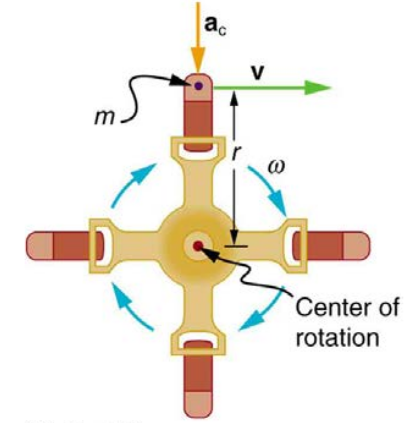
\includegraphics[width=0.25\textwidth]{figures/centrifuge.png}
\caption{\label{fig:cent} A centrifuge undergoes uniform circular motion, with tangential velocity $v$ and radius $r$.}
\end{figure}
\item A car traveling along a banked curve with radius $r$ is illustrated in Fig. \ref{fig:car}.  (a) Show that if the net force is zero as the car goes through this curve of radius $r$, that the speed of the car is $v = \sqrt{rg\tan\theta}$. (b) What is $v$, if $r=600$ m, $g\approx 10$ m/s$^2$, and $\theta = 10^{\circ}$?
\begin{figure}[ht]
\centering
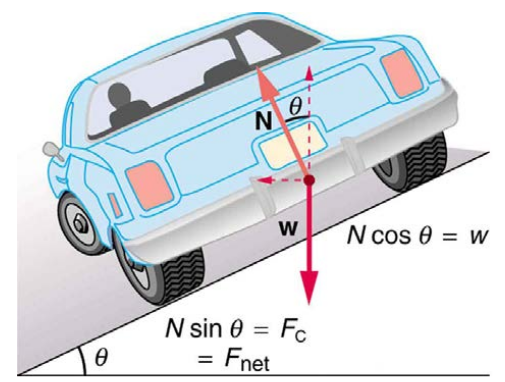
\includegraphics[width=0.25\textwidth]{figures/car.png}
\caption{\label{fig:car} A vehicle travels along a banked curve, hugging the road.}
\end{figure}
\end{enumerate}
\clearpage
\section{Newton's Law of Gravity}
\begin{enumerate}
\item Consider Fig. \ref{fig:planet}, in which a planet orbits a star.  Suppose that the acceleration due to gravity on the surface of the planet is $a$.  (a) Show that $a = GM_p/d^2$, where $G$ is Newton's constant.  (b)  What is $M_p$, if $a=7.6$ m/s$^2$, and $d = 5000$ km? (c) Show that if the period of the orbit of the planet around the star is $T$, that $M_S = 4\pi^2 b^3/T^2$. (d) If $b = 3 \times 10^{11}$ m (about 2 AU), and $T = 2$ years, what is $M_P$?
\begin{figure}[ht]
\centering
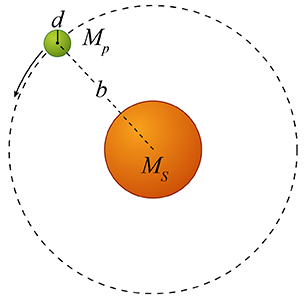
\includegraphics[width=0.25\textwidth]{figures/planet.png}
\caption{\label{fig:planet} A planet of mass $M_P$ and radius $d$ orbits a star of mass $M_S$ at an orbital radius $b$.}
\end{figure} \\ \vspace{0.5cm}
\item What is the orbital period of Neptune, $T_N$, if the orbital radius of Neptune, $r_N$, is 30 AU? (Recall that $T_{Earth} = 1.0$ year and $r_{Earth} = 1.0$ AU). \\ \vspace{1cm}
\end{enumerate}
\section{Work and the Work-Energy Theorem}
\begin{enumerate}
\item Consider Fig. \ref{fig:brief}.  (a) Explain in your own words why the work done \textit{on the briefcase} by the man is zero Joules for each case. (b) Now suppose there is work being done.  If the force vector is $\vec{F} = 3 \hat{i} + 3\hat{j}$ N, and $\vec{d} = 3\hat{i}$ m, what is the work $W$?
\begin{figure}[ht]
\centering
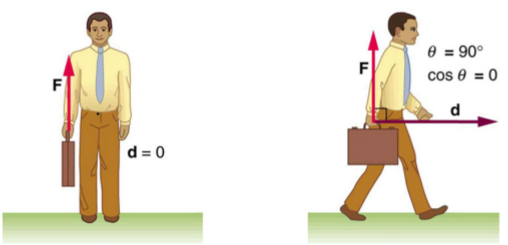
\includegraphics[width=0.4\textwidth]{figures/briefcase.png}
\caption{\label{fig:brief} A man holds a briefcase, with different displacements and forces.}
\end{figure}
\item (a) If a person throws a 0.145 kg baseball at $v=10$ m/s, what is the kinetic energy of the baseball?  (b) If a person drops a 0.145 kg baseball from a building that is 30 m tall, what is the final speed of the baseball? \\ \vspace{1cm}
\item What is the final velocity of the roller coaster cars in Fig. \ref{fig:coaster}?
\begin{figure}[ht]
\centering
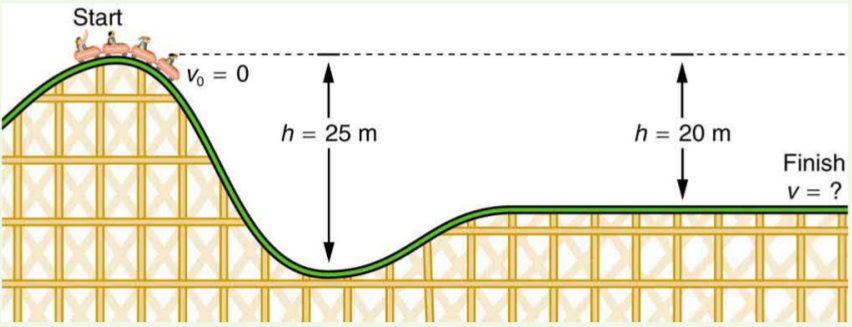
\includegraphics[width=0.5\textwidth]{figures/coaster.png}
\caption{\label{fig:coaster} A roller coaster starts with no initial velocity, but ends with velocity $v$.}
\end{figure}
\end{enumerate}
\end{document}